% =========================================================================
%  LunaLink ADCS Simulation Report
%  Project X, LunaLink Simulation Challenge
%  Spacecraft Design: Fundamentals, SS 2026, TUM
%
%  Compile from THIS directory (output/) so the figures resolve:
%      pdflatex LunaLink_ADCS_Report.tex
%      pdflatex LunaLink_ADCS_Report.tex   (second pass for references)
%
%  The figures are the PNG files produced by the headless run:
%      python -m lunalink.main_simulation
%  Regenerating the plots updates the report automatically on recompile.
% =========================================================================
\documentclass[11pt,a4paper]{article}

\usepackage[margin=2.2cm]{geometry}
\usepackage{graphicx}
\usepackage{amsmath,amssymb}
\usepackage{booktabs}
\usepackage{siunitx}
\usepackage{caption}
\usepackage[colorlinks=true,linkcolor=blue!50!black,urlcolor=blue!50!black,citecolor=blue!50!black]{hyperref}
\usepackage{microtype}

\graphicspath{{./}}
\captionsetup{font=small,labelfont=bf,skip=4pt}
\setlength{\parskip}{3pt}
\sisetup{per-mode=symbol}

\title{\vspace{-1.2cm}\textbf{LunaLink ADCS Simulation}\\[2pt]
\large Attitude Determination and Control for a Molniya-Orbit Earth--Moon Relay}
\author{Hemraj Chauhan\\
\small Project X, LunaLink Simulation Challenge \(\cdot\)
Spacecraft Design: Fundamentals, SS 2026, TUM}
\date{}

\begin{document}
\maketitle
\vspace{-0.9cm}

% -------------------------------------------------------------------------
\section{Introduction}

LunaLink is a \SI{500}{kg} relay spacecraft that connects a ground station
in Ottobrunn with a station on the Moon. It flies a Molniya-type orbit
(\(500 \times 36\,000\)~km, inclination \ang{63.4}). This report covers
the \textbf{ADCS}: the subsystem that measures and controls which way the
spacecraft points.

The simulation does four things. It sizes the actuators (reaction wheels
and magnetorquers). It models the space environment and the four
disturbance torques that act on the body along the orbit. It runs the
attitude control loop in four modes: detumbling, sun pointing, a combined
detumble-then-point mission, and a rest-to-rest slew. And it runs a simple
attitude estimator (gyro plus star tracker) next to the true state, so we
can tell apart how well the spacecraft \emph{knows} its attitude from how
well it \emph{controls} it.

The spacecraft is treated as a rigid body with reaction wheels. Its
rotation follows Euler's equation, and the attitude quaternion follows the
standard kinematics:
\begin{equation}
\mathbf{I}\,\dot{\boldsymbol\omega}
  = \mathbf{T}_{\mathrm{ext}} - \dot{\mathbf h}_w
  - \boldsymbol\omega \times \left(\mathbf{I}\boldsymbol\omega + \mathbf h_w\right),
\qquad
\dot{\mathbf q} = \tfrac{1}{2}\,\boldsymbol\Omega(\boldsymbol\omega)\,\mathbf q .
\label{eq:euler}
\end{equation}
These are integrated with a fixed-step RK4 scheme at
\(\Delta t = \SI{8}{s}\). The orbit itself is solved analytically from
Kepler's equation at every step, so there is no position drift from the
integrator. Both required scenarios run for \textbf{4 full orbits}, which
is \SI{42.7}{h} of simulated time and satisfies the brief requirement of
at least 3 orbits and at least \SI{36}{h}.

Two programs produce the results. A PyQt6 GUI shows a 3D orbit view, lets
the user change parameters, and updates all result plots live. A headless
script, \texttt{main\_simulation.py}, produces every figure in this report
with one command.

% -------------------------------------------------------------------------
\section{Assumptions}

Table~\ref{tab:assumptions} lists every engineering assumption and the
reason behind it.

\begin{table}[h]
\centering\small
\begin{tabular}{@{}p{3.4cm}p{5.2cm}p{6.6cm}@{}}
\toprule
\textbf{Assumption} & \textbf{Value / model} & \textbf{Why it is justified}\\
\midrule
Fixed Keplerian orbit & \(a=\SI{24628}{km}\), \(e=0.7207\),
  \(i=\ang{63.4}\), \(P=\SI{10.68}{h}\) &
  The main perturbation (J2) shifts the orbit plane by only
  \(-0.171\)\si{\degree\per\day} and the perigee by
  \(+0.0005\)\si{\degree\per\day} (\ang{63.4} is the critical
  inclination). Over the 1.8-day run that is under \ang{0.31}, so a fixed
  ellipse is accurate enough. Note: the brief's ``\(\approx\)12 h'' period
  does not match its own altitudes; we keep the altitudes, which give
  \SI{10.68}{h}.\\
Mass properties & uniform box: \(\mathbf I =
  \mathrm{diag}(135.4,\,208.3,\,260.4)\)~\si{kg.m^2} &
  Computed from \SI{500}{kg} and the \(2.0\times1.5\times1.0\)~m envelope
  with the standard box formula, as the brief asks.\\
CoM--CoP offset & \SI{0.10}{m} along body \(x\) &
  Solar pressure and drag need a lever arm to create torque; a
  \SI{10}{cm} offset is a typical conservative value.\\
Magnetic field & Earth dipole, \(M_B=\SI{7.94e15}{T.m^3}\) &
  The brief allows a dipole model. It captures the key physics: the field
  is strong at perigee and almost gone at apogee.\\
Atmosphere & exponential, \(\rho(\SI{500}{km})=\SI{e-12}{kg/m^3}\),
  scale height \SI{60}{km} &
  Drag only matters during the short perigee pass; above \SI{600}{km} it
  is switched off.\\
Eclipse and Sun & cylindrical Earth shadow; analytic Sun direction &
  Standard low-precision models; accurate enough for torque levels and
  eclipse timing.\\
Solar pressure & \(\Phi=\SI{1361}{W/m^2}\), \(A=\SI{3}{m^2}\),
  reflectance \(q=0.5\) & Flat-plate model with the SRP coefficient the
  brief asks us to state.\\
Residual dipole & \SI{1.0}{A.m^2} & Typical leftover magnetism of a small
  spacecraft; it produces the torque \(\mathbf m \times \mathbf B\).\\
Actuators & 3 wheels (\SI{4.0}{N.m.s}, \SI{0.05}{N.m} each);
  3 rods (\SI{50}{A.m^2}) & Sized in Sec.~\ref{sec:sizing}. Wheel torque
  and momentum limits are enforced in the simulation.\\
Sensors & gyro bias \((3,-2,1.5)\)\si{\degree\per\hour},
  noise \SI{e-6}{rad/s}; star tracker \SI{10}{arcsec} every \SI{20}{s} &
  Realistic values for commercial parts. The estimator stops learning the
  gyro bias while the spacecraft spins fast (see
  Sec.~\ref{sec:determination}).\\
Initial state & tumble of \SI{10}{\degree/s}; pointing starts \ang{12.5}
  off the Sun & The tumble rate is given in the brief.\\
Integration & RK4, \(\Delta t=\SI{8}{s}\) & Check: with all torques off,
  total angular momentum is conserved to \(10^{-15}\) relative error.\\
\bottomrule
\end{tabular}
\caption{Engineering assumptions.}
\label{tab:assumptions}
\end{table}

% -------------------------------------------------------------------------
\section{Results}

\subsection{Actuator sizing}\label{sec:sizing}

The wheels are sized by agility, not by disturbances. To turn \ang{90} in
\SI{300}{s} about the worst axis, the wheels must provide
\begin{equation}
T_{\mathrm{slew}} = \frac{4\,I\,\theta}{t^2} = \SI{18.2}{mN.m},
\qquad
h_{\mathrm{peak}} = \frac{T_{\mathrm{slew}}\, t}{2} = \SI{2.73}{N.m.s}.
\end{equation}
The disturbances only ask the wheels to store about \SI{0.13}{N.m.s} per
orbit, twenty times less. With a 1.5 margin on the slew value we select
\SI{4.0}{N.m.s} wheels with \SI{0.05}{N.m} torque.

For the magnetorquers, dumping the daily momentum build-up would need only
about \SI{0.02}{A.m^2}. Detumbling sets the real requirement: \SI{50}{A.m^2}
rods give about \SI{1.2}{mN.m} of control torque at perigee, where the
field is \(B \approx \SI{24}{\micro T}\). Table~\ref{tab:sizing} collects
the numbers.

\begin{table}[h]
\centering\small
\begin{tabular}{@{}lll@{}}
\toprule
\textbf{Quantity} & \textbf{Value} & \textbf{Set by}\\
\midrule
Principal inertia & 135.4 / 208.3 / 260.4 \si{kg.m^2} & 500 kg box\\
Slew control torque & \SI{18.2}{mN.m} & \ang{90} in \SI{300}{s}\\
Peak slew momentum & \SI{2.73}{N.m.s} & same slew\\
Disturbance storage & \SI{0.131}{N.m.s} per orbit & 4-orbit simulation\\
Selected wheel capacity & \SI{4.0}{N.m.s} (rec.\ 4.1) & slew + margin\\
Momentum to dump & \SI{0.241}{N.m.s} per day & solar pressure\\
Selected rod dipole & \SI{50}{A.m^2} & detumbling authority\\
\bottomrule
\end{tabular}
\caption{Sizing summary.}
\label{tab:sizing}
\end{table}

\subsection{Scenario 1: detumbling (4 orbits)}

After separation the spacecraft tumbles at \SI{10}{\degree/s}. The B-dot
law commands a magnetic dipole against the rotation,
\begin{equation}
\mathbf m = k\,(\boldsymbol\omega \times \mathbf B),
\qquad
\mathbf T_c = \mathbf m \times \mathbf B ,
\end{equation}
which always removes rotational energy
(\(\boldsymbol\omega^{\!\top}\mathbf T_c \le 0\)). The commanded dipole is
clipped at the \SI{50}{A.m^2} rod limit.

Figure~\ref{fig:detumble} shows the result: the rate falls from
\SI{10.1}{} to \SI{6.8}{\degree/s} in \SI{42.7}{h}, in clear steps. The
steps are the physics of this orbit. The control torque scales with
\(B^2\), and \(B\) falls with \(1/r^3\), so nearly all braking happens
during the short perigee pass. The long apogee arc contributes almost
nothing. Extrapolating the momentum removed per pass, a full detumble
takes roughly 10 to 12 orbits, about 4 to 5 days. This is a result, not a
flaw: it shows why missions in this kind of orbit either plan several days
for magnetic detumbling or carry thrusters for the first rate reduction.

\begin{figure}[h]
\centering
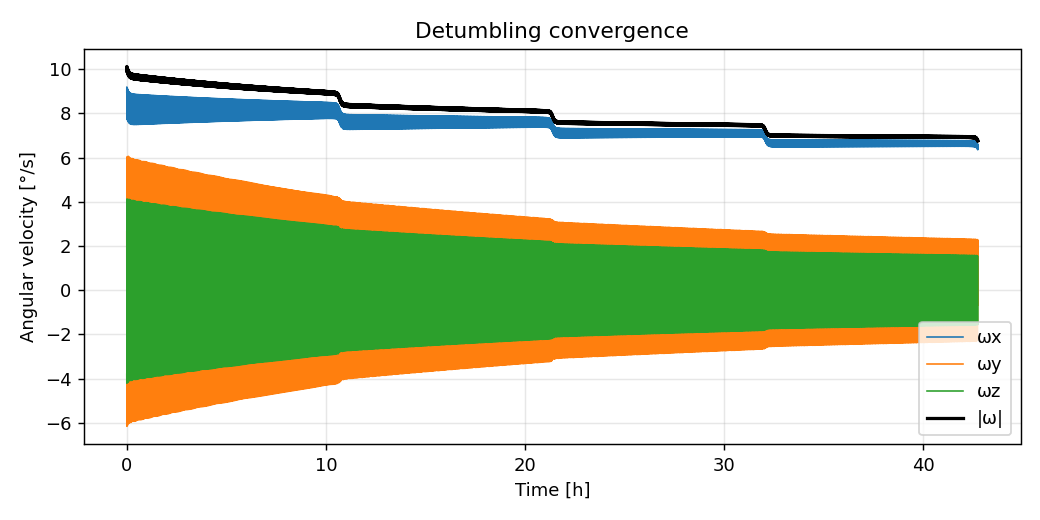
\includegraphics[width=0.86\textwidth]{detumble_angular_velocity.png}
\caption{Detumbling. The body rate drops in a step at every perigee pass,
because the magnetic field (and with it the control torque) is only strong
near perigee.}
\label{fig:detumble}
\end{figure}

\subsection{Scenario 2: sun pointing (4 orbits)}

The pointing controller is a quaternion PD law realised by the wheels:
\begin{equation}
\mathbf T_c = -\mathbf K_p\, \mathbf q_{e,v} - \mathbf K_d\, \boldsymbol\omega,
\qquad
\mathbf K_p = \mathbf I\,\omega_n^2,\quad
\mathbf K_d = 2\zeta\,\mathbf I\,\omega_n,
\end{equation}
with bandwidth \(\omega_n=\SI{0.05}{rad/s}\) and damping \(\zeta=0.7\).
Starting \ang{12.5} away from the Sun, the spacecraft locks on in about
\SI{2.6}{min} and then holds the Sun line for the rest of the run. The
final pointing error is \ang{0.020}; the RMS error over the settled part
of the run is \ang{0.0053} (Fig.~\ref{fig:pointing}).

\begin{figure}[h]
\centering
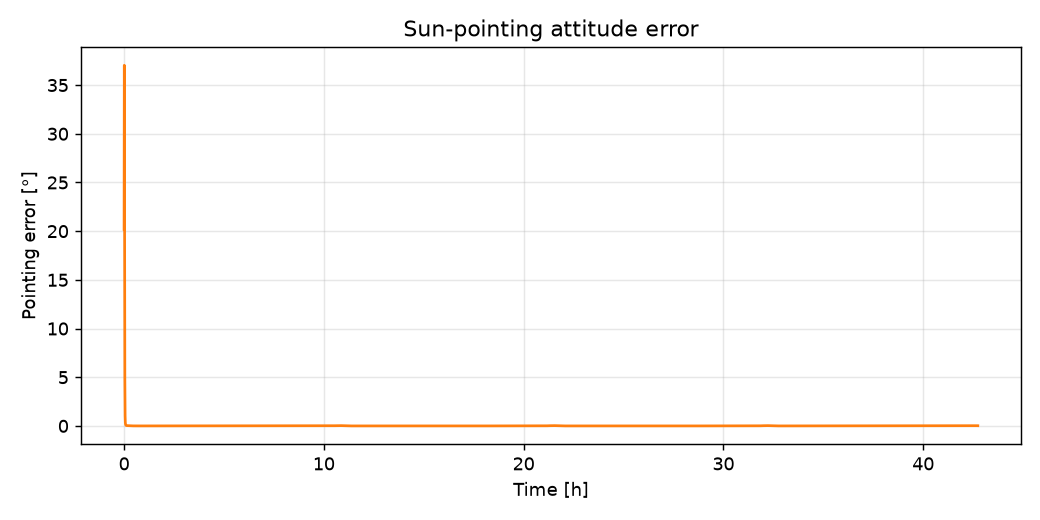
\includegraphics[width=0.86\textwidth]{sunpoint_attitude_error.png}
\caption{Sun-pointing error. Fast acquisition from the \ang{12.5} start,
then a hold below \ang{0.03} for four orbits.}
\label{fig:pointing}
\end{figure}

While pointing, the wheels slowly fill up with the momentum that the
steady part of the disturbance torque feeds into the body. When the stored
momentum crosses \SI{80}{\percent} of capacity (\SI{3.2}{N.m.s}), the
magnetorquers unload it with the cross-product law
\begin{equation}
\mathbf m = \frac{k_d}{\lVert\mathbf B\rVert^{2}}
            \left(\mathbf h_w \times \mathbf B\right)
\qquad\Rightarrow\qquad
\mathbf T_{\mathrm{mtq}} = -k_d\, \mathbf h_{w,\perp}.
\label{eq:desat}
\end{equation}
The torque opposes the stored momentum, so the wheels spin down. The sign
matters: with the cross product the other way round
(\(\mathbf B \times \mathbf h_w\)), the same law \emph{adds} momentum
instead of removing it (Sec.~\ref{sec:ai}). Because the field is weak away
from perigee, the unloading happens mostly during perigee passes, which
gives the slow saw-tooth in Fig.~\ref{fig:wheels}. Brief saturation at the
\SI{4.0}{N.m.s} per-wheel limit is visible and is handled consistently:
the torque applied to the body is computed from the momentum the wheels
can actually absorb.

\begin{figure}[h]
\centering
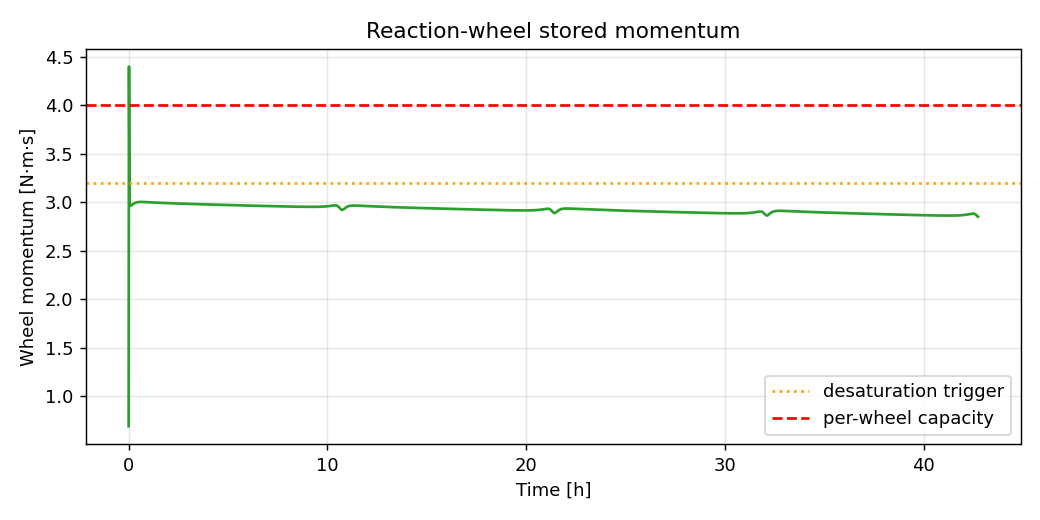
\includegraphics[width=0.86\textwidth]{sunpoint_rw_momentum.png}
\caption{Stored wheel momentum with the desaturation trigger
(\SI{3.2}{N.m.s}) and the per-wheel capacity (\SI{4.0}{N.m.s}).}
\label{fig:wheels}
\end{figure}

\subsection{Disturbance torques and the momentum budget}

Figure~\ref{fig:dist} ranks the four disturbance sources along the orbit.
Gravity gradient is the largest (peak \SI{1.6e-4}{N.m}) and spikes at
perigee because it scales with \(1/r^3\). The residual-dipole magnetic
torque (\SI{4.5e-5}{N.m}) and air drag (\SI{7.6e-6}{N.m}, only below
\SI{600}{km}) also peak at perigee. Solar pressure is the smallest
(\SI{2.0e-6}{N.m}) but it is the only torque that does not average out
over an orbit, so it alone sets how much momentum must be dumped per day:
\SI{0.24}{N.m.s}. Figure~\ref{fig:budget} shows this directly: the
per-orbit wiggle is momentum the wheels borrow and give back; the steady
climb is what the magnetorquers must remove.

\begin{figure}[h]
\centering
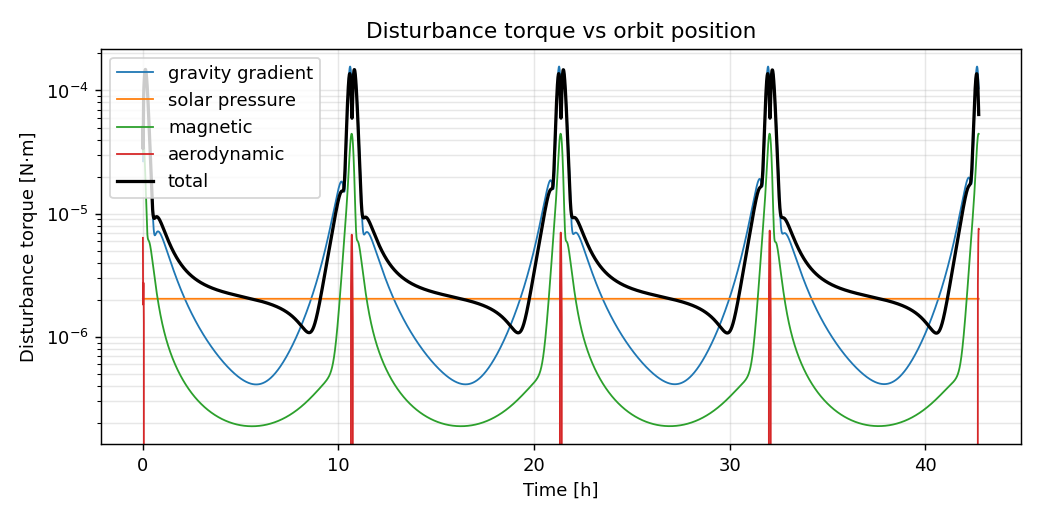
\includegraphics[width=0.86\textwidth]{sunpoint_disturbance_torque.png}
\caption{Disturbance torques along the orbit (log scale). Gravity gradient
dominates at perigee; solar pressure carries the steady load near apogee.}
\label{fig:dist}
\end{figure}

\begin{figure}[h]
\centering
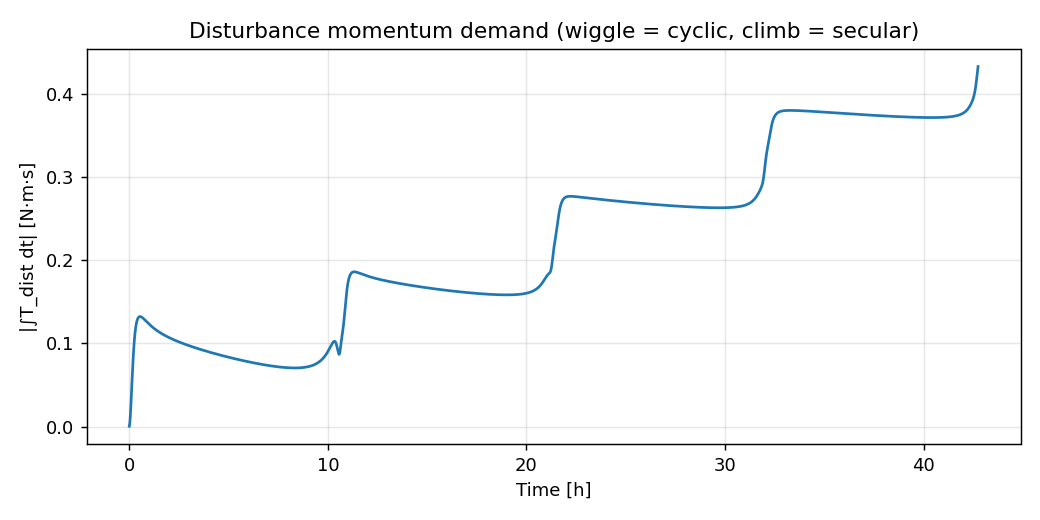
\includegraphics[width=0.86\textwidth]{sunpoint_momentum_budget.png}
\caption{Accumulated disturbance momentum. Wiggle = cyclic (wheels store
it), climb = secular (torquers dump it).}
\label{fig:budget}
\end{figure}

\subsection{Attitude determination and the pointing budget}
\label{sec:determination}

The estimator combines two sensors. The gyro is fast but drifts because of
its bias; the star tracker is absolute but slower and noisier per sample.
A complementary filter integrates the gyro between star fixes, and each
fix pulls the estimate back and updates the bias estimate:
\begin{equation}
\mathbf a = 2\,\mathrm{vec}\!\left(\hat{\mathbf q}^{-1}\otimes
\mathbf q_{\mathrm{meas}}\right),
\qquad
\hat{\mathbf q} \leftarrow \hat{\mathbf q}\otimes
\delta\mathbf q(k_p\,\mathbf a),
\qquad
\hat{\mathbf b} \leftarrow \hat{\mathbf b} - k_i\,\mathbf a / T .
\end{equation}
The filter learns the gyro bias from \SI{3.91}{} down to
\SI{0.25}{\degree\per\hour}, and the knowledge error settles at the star
tracker noise floor (Fig.~\ref{fig:det}).

The resulting pointing budget, evaluated over the settled part of the run:
knowledge error \ang{0.0045} RMS (budget \ang{0.01}, \textbf{pass}),
control error \ang{0.0053} RMS (budget \ang{0.08}), total \ang{0.0098}
against the \ang{0.1} allocation. One practical detail: during detumbling
the bias update is paused. With \SI{20}{s} between star fixes at
\SI{10}{\degree/s}, the spacecraft turns more than \ang{180} between
fixes, so the measured residual no longer reflects the bias and would
corrupt the estimate.

\begin{figure}[h]
\centering
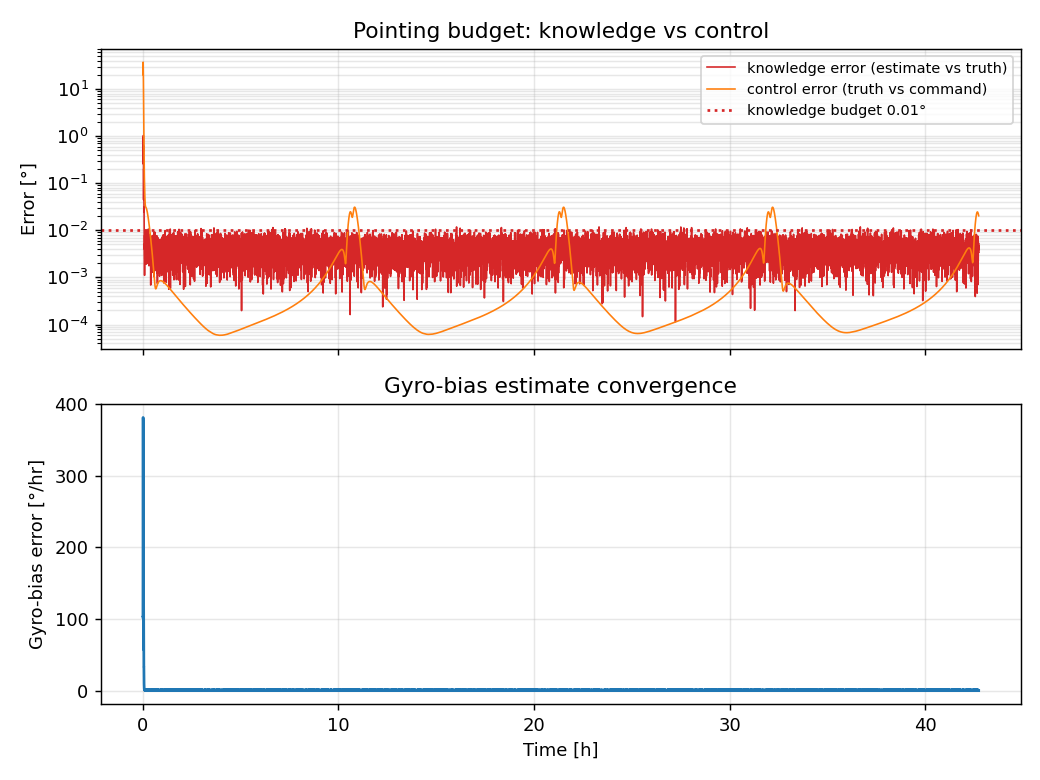
\includegraphics[width=0.86\textwidth]{sunpoint_pointing_budget.png}
\caption{Top: knowledge vs control error (log scale). Bottom: the gyro
bias estimate converging.}
\label{fig:det}
\end{figure}

% -------------------------------------------------------------------------
\section{How AI was used}\label{sec:ai}

I used Claude (Anthropic) throughout the project, and always checked its
output independently.

\textbf{Code review.} The AI went through every formula against SMAD and
the lecture notes. It found three real bugs, which I checked and then
fixed: the desaturation law had the cross product reversed, which pumps
momentum \emph{into} the wheels instead of out (the correct form is
Eq.~\eqref{eq:desat}); the initial pointing offset used \(\sin\theta\)
where a quaternion needs the half angle \(\sin(\theta/2)\), so the start
offset was twice what was configured; and the bias estimator diverged
during detumbling because the spacecraft rotates more than \ang{180}
between star fixes.

\textbf{Verification.} The AI wrote numerical checks that I ran and kept:
momentum conservation without torques (\(10^{-15}\)), round-trip tests of
the quaternion conventions, and regression tests that pin all result
numbers so refactoring cannot silently change the physics.

\textbf{Engineering work.} Refactoring the code into a clean physics/GUI
structure, the PyQt6 interface, plot design, documentation, and the draft
of this report.

\textbf{What I had to correct.} The AI's first fix for the estimator
(rejecting large residuals) did not stop the divergence, because the
aliased residuals \emph{look} small. The working fix gates on the expected
rotation between fixes instead. All final numbers in this report come from
the committed code and are reproduced with one command.

% -------------------------------------------------------------------------
\section{References}

\begin{enumerate}\itemsep1pt
\item J.~R. Wertz, D.~F. Everett, J.~J. Puschell (eds.),
      \emph{Space Mission Engineering: The New SMAD}, Microcosm Press,
      2011. (Slew torque, cyclic storage and dipole sizing equations.)
\item F.~L. Markley, J.~L. Crassidis, \emph{Fundamentals of Spacecraft
      Attitude Determination and Control}, Springer, 2014. (Quaternion
      conventions, Euler equation with wheels, complementary filtering.)
\item D.~A. Vallado, \emph{Fundamentals of Astrodynamics and
      Applications}, 4th ed., Microcosm Press, 2013. (Kepler propagation,
      J2 secular rates, solar ephemeris.)
\item M.~J. Sidi, \emph{Spacecraft Dynamics and Control}, Cambridge
      University Press, 1997. (B-dot detumbling, cross-product
      desaturation law.)
\item TUM Chair of Spacecraft Systems, \emph{Spacecraft Design:
      Fundamentals SS 2026}, ADCS lecture and exercise notes.
\item \emph{Project X, LunaLink Simulation Challenge brief}, v2, TUM,
      2026.
\end{enumerate}

\end{document}
